\chapter{Stato dell'arte}
\label{cha:statoArte}

\section{Reverse Proxy}
\begin{figure}[h!]
  \centering
  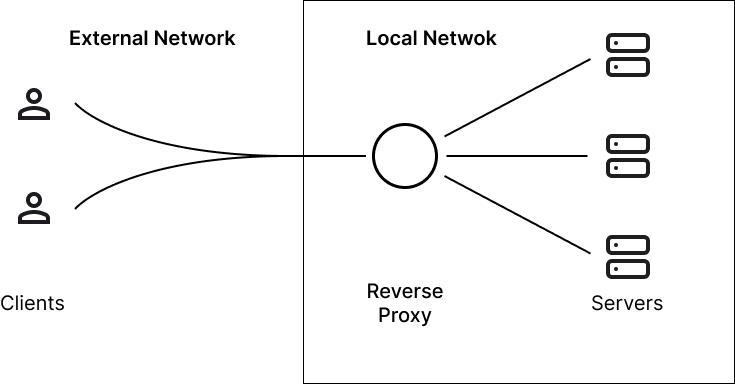
\includegraphics[width=.6\textwidth]{images/schema.png}
\end{figure}

\subsection{Cos'é}
Un reverse proxy é server che si pone in mezzo tra i server e i client. Le comunicazioni che quindi verranno effettuate tra questi 2 nodi, passeranno tutte attraveso il reverse proxy. Avendo accesso a tutte le comunicazioni, questo dispositivo puó effettuare dei test di sicurezza per assicurarsi che le richieste non siano maligne.

\subsection{Esempio comunicazione}
\textit{Client: A, Reverse proxy: R, Server: B}
\begin{enumerate}
  \item A invia un messaggio R, in cui peró specifica a quale server vuole collegarsi (questo viene effettuato tramite l'assegnazione di un subdomain specifico per ogni server).
  \item R riceve la comunicazione, controlla a quale server é indirizzata e effettua una richiesta uguale a quella ricevuta peró cambiando il destinatario che in questo caso sará il server effettivo.
  \item B riceve la richiesta, elabora la risposta ed invia a R la risposta.
  \item R riceve la risposta e la invia ad A

\end{enumerate}

\subsection{Perché viene utilizzato}
L'utilizzo di una struttura che si pone in mezzo alle comunicazioni garantisce molti vantaggi visto che ha accesso a tutte le comunicazioni entranti. Il reverse proxy puó quindi analizzare le connessioni ed effettuare delle operazioni con queste ultime come ad esempio controlli per motivi di sicurezza, chaching e load balancing. Inoltre in questo modo si puó accedere a piú servizi tramite lo stesso nodo di ingresso.

\subsection{Funzionalitá}
Analizziamo adesso le funzionalitá che un reverse proxy puó offrire.

\subsubsection{Sicurezza}
Sicuramente le funzionalitá piú importanti sono quelle relative alla sicurezza. Un reverse proxy infatti ne implementa molte evitando la necessitá di implementare sistemi di sicurezza per ogni servizio che andiamo ad inserire nella rete locale.
\begin{enumerate}
  \item \textbf{TLS}: Ogni comunicazioni in ingresso e in uscita puó essere criptata tramite il protocollo TLS.
  \item \textbf{controllo attacchi DoS/DDoS}: Controllando tutte le comunicazioni e i relativi ip sorgente, si possono applicare filtri e controlli per evitare un eccesso di richieste in entrata che possono rallentare le funzionalitá dei server.
  \item \textbf{supporto protocolli piú recenti}: Il reverse proxy puó supportare protocolli piú recenti rispetto ai server cosí la connessione interna tra servere e reverse proxy puó essere effettuata nel protocollo piú recente supportata dal server, ma poi quella all'esterno puó essere elevata ad un protocollo piú recente e quindi con maggiore sicurezza.

\end{enumerate}

\subsubsection{Prestazioni}
\begin{enumerate}
  \item \textbf{TLS}: Criptare la comunicazione nel nodo del reverse proxy e lasciando la comunicazione interna in chiaro allegerisce molto il carico di lavoro ai server.
  \item \textbf{Cache}: Implementando un sistema di caching, richieste ricorrenti alle stesse risorse possono essere soddisfatte direttamente dal reverse proxy, senza inoltrare la richiesta al server.
  \item \textbf{Compressione}: Comprimere le risposte cosí da occupare meno banda e non influire sulle prestazioni dei server in quanto il processo di compressione e decompressione delle richieste é effettuato dal reverse proxy.
\end{enumerate}

\subsubsection{Load Balancer}
Se si hanno piú server (macchine) che rispondono alle stesse richieste, si possono indirizzare le richieste in modo che carico di lavoro sia distribuito equamente tra i vari server. In base all'algoritmo implementato il processo di load balancing puó essere fatto in modo accurato oppure piú grezzo. L'algoritmo scelto dipende molto dal caso d'uso.

\section{SSL/TLS}
SSL/TLS é il protocollo utilizzato per criptare le comuncazioni web, sia che si utilizzi https che wss (Secure WebSocket). SSL é la versione vecchia di questo protocollo che ormai non viene piú utilizzata perché usa protocolli troppo deboli rispetto alle capacitá computazionali odierne. Quindi un messaggio criptato tramite SSL ora verrebbe decriptata in relativa rapiditá. Questo rende la connessione non sicura. TLS inevece é il protocollo nuovo, che ora ha raggiunto la versione 1.3 che é considerato sicuro e difficilmente decriptabile con le tecnologie odierne.
\subsection{Funzionamento}
\subsubsection{Handshake}
Quando viene instaurata la connessione i primi messaggi inviati dalle due parti servono per effettuare l'handshake. Durante questa fase si vanno a decidere protocolli utilizzati, chiavi, nonce.
\begin{enumerate}
  \item \textbf{fase 1}: Nella prima fase si negoziano la versione di TLS da utilizzare e i nonce, succesivamente utilizzate per identificare la sequenza dei messaggi.
  \item \textbf{fase 2}: Il server invia al client la chiave pubblica per verificare il certificato e la sua parte di parametri in caso venga utilizzato DH come protocollo di condivisione della chiave.
  \item \textbf{fase 3}: Il client tramite la chiave pubblica del certificato verifica che il server é il vero possessore del certificato e invia al server is suoi parametri in caso di DH, oppure la chiave criptata con la chiave pubblica del server in caso di RSA.
\end{enumerate}
\subsubsection{Record}
I messaggi dopo quelli di handshake verranno poi criptati e verificato che non siano stati modificati.
\begin{enumerate}
\item \textbf{confidenzialitá}: il contenuto del messaggio deve essere visibile solamente alle 2 parti, se non si ha possesso delle chiavi non é possibile leggere il contenuto in chiaro.
\item \textbf{integritá}: se il messaggio é stato modificato nel mezzo della comunicazione, questo deve essere identificabile. Per effettuare ció si calcola il valore hash del messaggio e si cripta tramite una chiave negoziata. Il ricevente calcolerá poi il valore hash del messaggio ricevuto e se i 2 valori combaciano vuol dire che il messaggio non é stato modificato.
\end{enumerate}

\section{Container}
\subsection{Cosa sono}
\cite{container}I container sono software eseguibili che contengono tutte le dipendenze per essere eseguiti come librerie, binari e file di configurazione. Indipendentemente dal sistema "host", cioé il sistema su cui viene eseguito il container, quest'ultimo funzionerá sempre allo stesso modo. Per uno sviluppatore questo é molto importante perché altrimenti dovrebbe creare delle versioni diverse dello stesso software per adattarle a ogni tipo di sistema operativo.
\subsection{Differenze dalle macchine virtuali}
\begin{enumerate}
  \item \textbf{kernel}: I container si appoggiano sul kernel del sistema operativo ospitante, mentre le macchine virtuali sono un sistema operativo che gira sopra il sistema operativo ospitante, con anche l'hardware che viene simulato. Questa differenza rende i container molto piú leggeri sia come utilizzo di risorse che come dimensione effettiva del software.
  \item \textbf{isolamento}: I container isolano il software a livello di processo, mentre le chiamate kernel fanno affidamento al sistema operativo ospitante. Le macchine virtuali invece non condividono niente col sistema operativo ospitante in quanto un nuovo sistema operativo é emulato per intero. Questo maggiore isolamento peró non é necessario nella maggiore parte dei casi, almeno che non vengano utilizzate queste tecnologie per offrire dei servizi dove gli utenti posson eseguire del codice all'interno dell'ambiente virtualizzato. In questo caso é meglio avere l'ambiente completamente isolato.
\end{enumerate}

\subsection{Docker}
\cite{docker}Docker é attulamente il software maggiormente utilizzato per la creazione, gestione ed esecuzione dei container. La sua popolaritá é dovuta principalmente alla semplicitá di utilizzo e alla gestione dei container. Infatti per creare un container bisogna creare un file dove vengono scritte le direttive per compilare il progetto e i comandi da eseguire quando il container viene eseguito. La gestione risulta inoltre comoda in quanto c'é un sistema di versionamento dei container, in stile git, che rende la gestione delle versioni comoda.

\subsection{Kubernetes}
Kubernetes é un ulteriore software che rende la scalabilitá dei container piú facile ed efficiente. Con kubernetes infatti si possono eseguire dei servizi utilizzando le risorse di diverse macchine. Quindi se si hanno molteplici macchine e un servizio molto difficile da eseguire, tramite kubernetes si possono dividere le operazioni su queste macchine.
